% !TEX encoding = UTF-8
% !TEX TS-program = pdflatex
% !TEX root = ../tesi.tex
% !TEX spellcheck = it-IT

%**************************************************************
\chapter{Il progetto nella strategia aziendale}
\label{cap:processi-metodologie}
%**************************************************************

\intro{Questo capitolo intende fornire una descrizione dettagliata del progetto di stage e dei motivi che hanno spinto l'azienda a proporlo oltre che i benefici derivati da tale progetto. Nel capitolo discuto anche i vincoli tecnologici e metodologici che l'azienda ha imposto sul mio stage}\\

%**************************************************************
\section{Presentazione del progetto}
Il progetto di stage riguarda la realizzazione di un motore di raccomandazione basato sul guadagno informativo negli alberi decisionali. Il sistema deve consentire il salvataggio del comportamento dell'utente, all'interno di un sito, e costruire un albero attraverso la classificazione dell'appartenenza di un oggetto ad una classe (immagini cliccata o non cliccata, \textit{hover}, ecc.). Questo tipo di apprendimento deve funzionare anche per gli esempi non ancora forniti al sistema: solamente dall'osservazione di fatti e oggetti relativi all'ambiente circostante, il sistema deve generalizzare i dati e le informazioni ricevute, ottenendo conoscenza che, auspicalmente, sia valida anche per i casi non ancora osservati.\\
Un albero decisionale è un piano strutturato ad albero che individua una successione di test sugli attributi noti e cioè il comportamento dell'utente al fine di predire un attributo  di output e cioè la raccomandazione. Prima della creazione dell'albero bisogna stabilire quali test effettuare su quali attributi. Ad ogni passo della creazione dell'albero, l'algoritmo deve scegliere su quale attributo fare lo \textit{split}.\\
Ad esempio un albero decisionale per decidere  se è la giornata ideale per giocare a tennis è il seguente:
\begin{figure}[h]
\centering
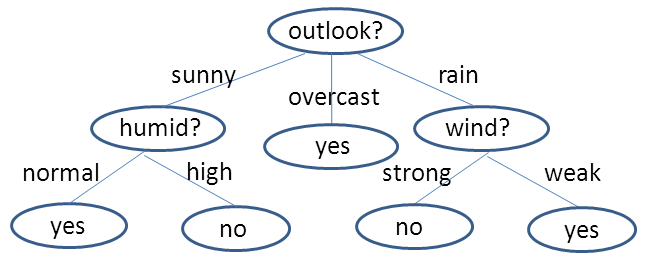
\includegraphics[width=0.7\linewidth]{immagini/play}
\caption[Esempio di albero decisionale]{Esempio di albero decisionale}
\label{fig:albero-decisionale-esempio}
\end{figure}

\newpage
\subsection{Obiettivi dello stage}
Lo stage ha una durata prevista di 300-320 ore complessive. Prima dell'inizio dello stage, \textbf{Nextep }ha redatto il \textit{Piano di Lavoro }contenente tutti gli obiettivi da realizzare nelle settimane di stage.
Gli obiettivi dello stage erano suddivisi in obiettivi minimi e obiettivi massimi. Durante le settimane  di lavoro essi hanno subito delle modifiche dovute alla strategia aziendale e dalle priorità del team di sviluppo. In un primo momento, infatti, è stato fatto il \textit{porting }da \textit{MongoDB a OrientDB }e l'\textit{upgrade }di versione del \gls{framework} Play di un progetto preesistente chiamato DRE. Questo ha comportato un ritardo di quanto pianificato e il lavoro è stato sospeso per realizzare il nuovo modulo Tres.\\
Di seguito sono riportati gli obiettivi dello stage:
\begin{itemize}
	\item \textbf{Obiettivi formativi:}
	\begin{itemize}
		\item Formazione sui sistemi di raccomandazione e degli algoritmi di apprendimento;
		\item Studio delle tecnologie utilizzate, Scala e OrientDB;
		\item Studio degli strumenti utilizzati, in particolar modo del \gls{framework} e degli \gls{IDE}.
	\end{itemize}
	\item \textbf{Obiettivi minimi:}
	\begin{itemize}
		\item Utilizzo del \textit{database} OrientDB.
	\end{itemize}
	\item \textbf{Obiettivi massimi:}
	\begin{itemize}
		\item Implementazioni di nuovi modelli di algoritmi di apprendimento per migliorare l'individuazione dei gusti dell'utente;
		\item Migliorare la fase di apprendimento del modello stesso;
		\item Implementazioni di algoritmi di \textit{cluster }per il raggruppamento di elementi omogenei in un insieme di dati.
	\end{itemize}
\end{itemize}

\subsection{Motivazioni}
La motivazione che spinge l'azienda a investire sugli stagisti è la possibilità di entrare in un settore di mercato differente dalle loro attività principali. Con lo scopo di capire se l'idea è utile e vantaggiosa, si creano le opportunità di stage durante i quali gli stagisti si prendono l'impegno di sviluppare un prodotto con le funzionalità attese dall'azienda; tuttavia non è escluso un possibile inserimento nel proprio organico dello stagista, infatti, l'azienda, attraverso l'attivazione di tirocini, avrà la possibilità di individuare, di valutare e di formare i futuri soggetti da inserire all'interno dell'azienda, superando quella che è la fase più dispendiosa.\\
Il progetto di stage rientra in una strategia aziendale che punta a rilasciare nuove funzionalità per i progetti attivi. In particolare si è costatato che una grande parte delle attività era la gestione di notevoli quantità di dati. Ciò rende il problema della gestione e dell'organizzazione di questa mole informativa una questione quantomai prioritaria, che cerca soluzioni nuove e facilitano l'esperienza utente. \textit{Nextep} vuole sfruttare questi dati e fornire un servizio di raccomandazione attraverso la classificazione del comportamento dell'utente, con l'aiuto di un albero decisionale, all'interno di un sito. Con il rilascio, l'azienda vuole fornire un servizio di tipo \textit{Software as a service} (SaaS), attraverso il quale fornirà all'utente la possibilità di gestire autonomamente i contenuti.\\
L'obiettivo principale dello stage consta nel realizzare un prototipo del prodotto.

\section{Vincoli di progetto}

\subsection{Vincoli del dominio}
Il sistema da realizzare deve riuscire a gestire una grande quantità di dati e l'architettura deve permettere di scalare facilmente e deve avere un'alta affidabilità. Per questo viene usato OrientDB come \textit{database} nella sua versione a grafo. Un database a grafo è simile a una struttura a rete composto da nodi e spigoli. OrientDB permette di scalare il database all'aumentare dei dati attraverso lo \textit{sharding}, usando \textit{cluster} multipli per classe, in cui ogni \textit{cluster} ha una propria lista di \textit{server} dove replicare i dati.
\begin{figure}[h]
\centering
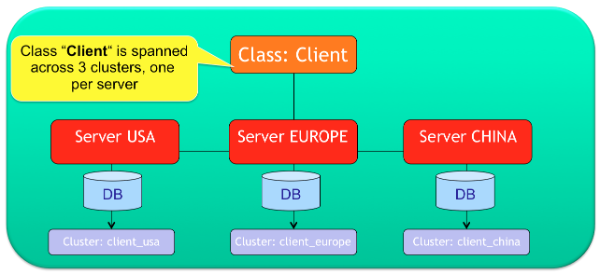
\includegraphics[width=0.9\linewidth]{immagini/distributed-sharding-class}
\caption[Esempio classe "Client" diviso in 3 clusters]{Esempio classe "Client" diviso in 3 \textit{clusters}. Questa immagine è stata presa dalla documentazione ufficiale di \href{http://orientdb.com/docs/last/Distributed-Sharding.html}{OrientDB}}
\label{fig:distributed-sharding-class}
\end{figure}

\subsection{Vincoli tecnologici}
\subsubsection*{Play framework}
Per lo sviluppo dell'applicativo è stato utilizzato il \gls{framework} Play\footnote{\url{https://www.playframework.com/documentation/2.4.x/Home}}. Esso è scritto in Scala e permette lo sviluppo delle \textit{web application} concorrenti, distribuite e altamente scalabili. \\
Play consente di ottimizzare lo sviluppo permettendo di ricaricare le classi modificate senza dover riavviare il server, ma solamente ricaricando le pagine dal \textit{browser}.\\
Le caratteristiche principali di Play sono:
\begin{itemize}
	\item Permette la visualizzazione degli errori direttamente dal \textit{browser};
	\item Utilizza il \textit{design pattern} \gls{mvc}\footnote{\url{https://www.playframework.com/documentation/1.0/main}};
	\item Possiede un motore di \textit{template} per le pagine HTML in linguaggio Scala;
	\item Rende facile la realizzazione di servizi \gls{REST}. \gls{REST} utilizza un aggregato di dati con un nome(\gls{URI}) e una rappresentazione, in questo caso \gls{JSON}, su cui è possibile invocare operazioni \textit{CREATE, READ, UPDATE, DELETE} (CRUD). Le associazioni tra richieste e \textit{controller} sono tutte mappate all'interno del file \textit{route} presente in tutti i progetti Play;
	\item Fornisce delle classi per facilitare la manipolazione di oggetti \gls{JSON};
	\item Permette di gestire facilmente le dipendenze verso librerie esterne sviluppate da terzi attraverso il file SBT\footnote{\url{http://www.scala-sbt.org/index.html}} contenente tutte le dipendenze del progetto;
	\item Fornisce librerie per realizzare i test su quanto sviluppato.\footnote{\url{https://www.playframework.com/documentation/2.0/ScalaTest}}
\end{itemize}
Tutte le richieste HTTP vengono gestite da Play nel modo seguente:
\begin{itemize}
	\item Il \gls{framework} riceve la richiesta HTTP;
	\item Viene cercato nel file \textit{route} l'azione del \textit{controller} corrispondente alla richiesta;
	\item Il codice del \textit{controller} viene eseguito;
	\item Se necessario il \textit{controller} genera una \textit{view} da ritornare al chiamante;
	\item Il \textit{controller} restituisce una risposta HTTP.
\end{itemize}
\begin{figure}[h]
\centering
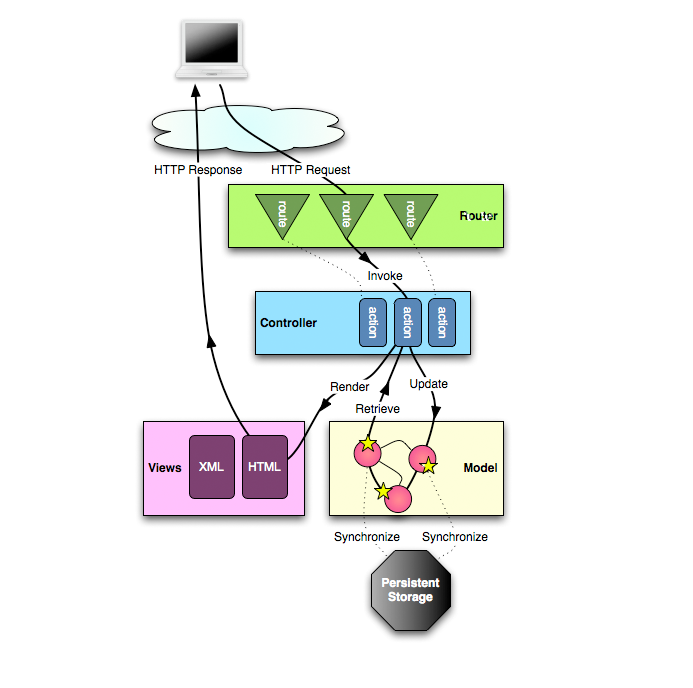
\includegraphics[width=0.8\linewidth]{immagini/diagrams_path}
\caption[Gestione di una richiesta HTTP in Play]{Gestione di una richiesta HTTP in Play. Questa immagine è stata presa dalla documentazione ufficiale di \href{https://www.playframework.com/documentation/1.0/main}{\textit{Play Framework}}}
\label{fig:diagrams_path}
\end{figure}

\newpage
\subsection*{OrientDB}
Come DBMS per il salvataggio dei dati si è scelto di utilizzare OrientDB\footnote{\url{http://orientdb.com/}}, nella sua versione di tipo \textit{graphdatabase}. Riesce a modellare ogni tipo di dominio, anche complesso, come un grafo, dove ogni entità è un \textit{Vertex},vertice in italiano, e tutte le relazioni sono \textit{Edge}, spigoli.
\begin{figure}[h]
\centering
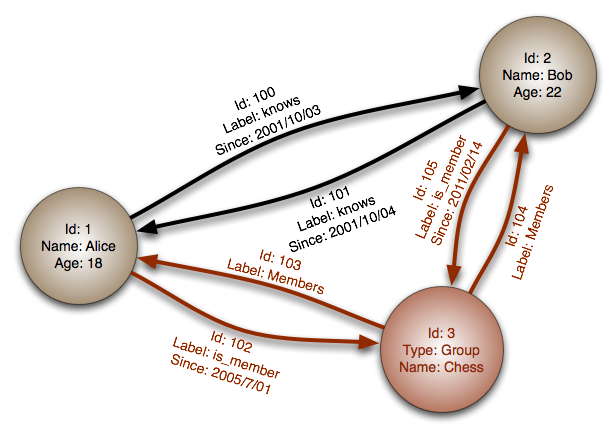
\includegraphics[width=0.8\linewidth]{immagini/GraphDatabase_PropertyGraph}
\caption[Esempio modellazione in OrientDB]{Esempio modellazione in OrientDB. Questa immagine è stata presa dall'\href{https://en.wikipedia.org/wiki/Graph_database}{articolo sui \textit{database} a graffo di Wikipedia}}
\label{fig:GraphDatabase_PropertyGraph}
\end{figure}

Le caratteristiche chiave di OrientDB sono:
\begin{itemize}
	\item Multiple modalità di \textit{storage: document, graph}(con supporto allo \textit{stack} Tinkerpop\footnote{\url{http://tinkerpop.incubator.apache.org/}}), \textit{object, key/value};
	\item Funzionamento \textit{embedded, in memory, client/server};
	\item Fornisce le proprietà ACID (Atomicità, Coerenza, Isolamento e Durabilità) di consistenza delle transizioni;
	\item Supporta nativamente \gls{JSON} e \gls{REST};
	\item È scritto in Java e quindi può girare su moltissime piattaforme.
\end{itemize}
Le caratteristiche che hanno portato alla scelta di OrientDB sono:
\begin{itemize}
	\item \textbf{Niente più join}: si può utilizzare il concetto di oggetti embedded ma supporta anche le relazioni senza l'uso del costoso \textit{JOIN}. Al contrario OrientDB usa i puntatori tra \textit{records}. Nella seguente immagine si può osservare la relazione tra due \textit{record} usando l'id \#8:124 per connettere \textit{Order} con \textit{Customer}.
	\begin{figure}[h]
	\centering
	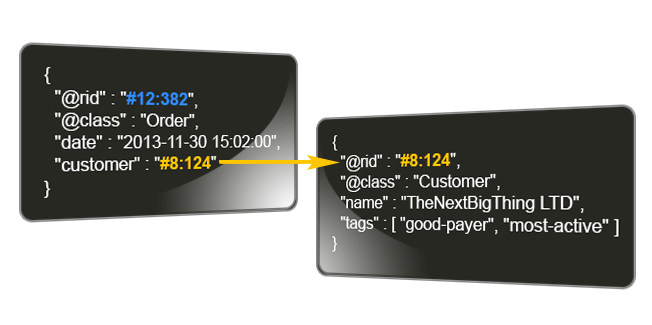
\includegraphics[width=0.8\linewidth]{immagini/json_linked3}
	\caption[Relazione tra due documenti]{Relazione tra due documenti. Questa immagine è stata presa dal sito ufficiale di \href{http://orientdb.com/orientdb-vs-mongodb/}{OrientDB}}
	\label{fig:json_linked3}
	\end{figure}
	

\item \textbf{Pensato per i big data}: con i database relazionali e documentali, più dati abbiamo, più lento diventa. OrientDB gestisce le relazioni come dei \textit{link} fisici ai \textit{records}. Questi vengono assegnati un'unica volta alla creazione del \textit{Edge} in tempo O(1);
\item \textbf{Scalabile:} OrientDB è un database scalabile. All'aumentare della dimensione del \textit{database} è possibile suddividere i dati del db in parti dette \textit{shard}, semplicemente aggiungendo un nodo nella rete che sarà automaticamente accettato dal \textit{server} distribuito senza bisogno di configurazioni. Le sincronizzazioni saranno automatiche non appena il \textit{server} sarà online;
\begin{figure}[h]
\centering
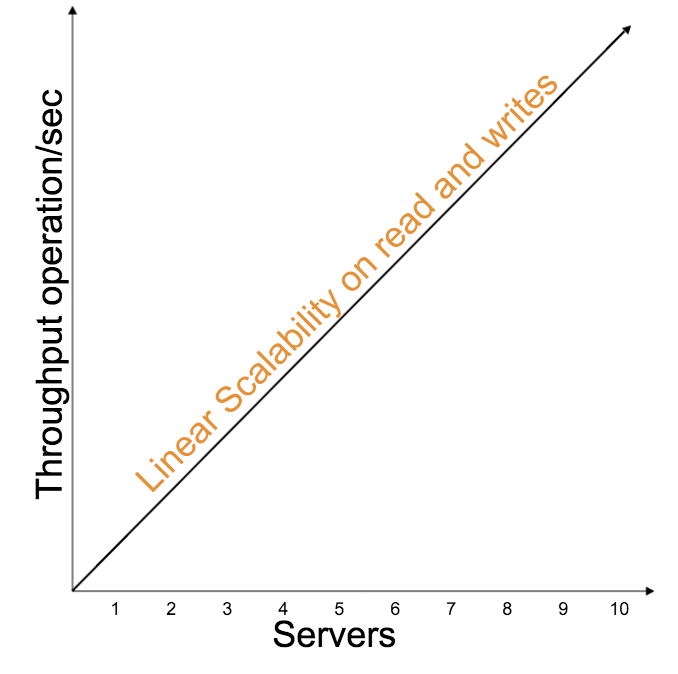
\includegraphics[width=0.7\linewidth]{immagini/rapporto-scalabilita}
\caption[Rapporto scalabilità]{Rapporto scalabilità}
\label{fig:rapporto-scalabilità}
\end{figure}


\item \textbf{Ripristino dati in caso di crash:} grazie a WAL (\textit{Write Ahead Logging}), OrientDB è capace di ripristinare il contenuto del database in caso di \textit{crash}. Tutte le transazioni in pendenza tornano allo stato in cui erano prima che le modifiche venissero apportate e tutti i cliente connessi al nodo vengono automaticamente spostati su un nodo \textit{server} disponibile.
\end{itemize}
La versione utilizzata durante lo stage è \textit{"orientdb-community-2.1.5"}. Per interagire con il \textit{database} si è scelto di utilizzare le Java \gls{api} nella versione \textit{graph} \gls{api}.

\subsection*{Scala}
Il linguaggio di programmazione scelto per lo sviluppo è Scala\footnote{\url{http://www.scala-lang.org/}}. È un linguaggio per la \gls{JVM} staticamente tipato, a paradigma misto. Cerca di unire la programmazione ad oggetti con la programmazione funzionale, permettendo a seconda della situazione, di scegliere l'approccio più adatto a soddisfare le esigenze.  Scala semplifica certi problemi di progettazione, in particolare quelli legati alla concorrenza. I linguaggi funzionali \textit{"puri"} non permettono alcun stato mutabile, evitando di conseguenza il bisogno di sincronizzazione sull'accesso condiviso allo stato mutabile. Invece, i programmi scritti in linguaggi puramente funzionali comunicano scambiando messaggi tra processi autonomi e concorrenti. Scala supporta questo modello con la sua libreria di attori, ma consente di usare variabili mutabili e immutabili.\\
Le funzioni sono cittadini \textit{"di prima classe"} nella programmazione funzionale, nel senso che possono essere assegnate a variabili, passate ad altre funzioni, esattamente come gli altri valori. Questa caratteristica promuove la composizione di comportamenti avanzati usando operazioni primitive. Dato che Scala aderisce al principio per cui ogni cosa è un oggetto, in Scala anche le funzioni sono oggetti.\\ Il linguaggio ha una sintassi molto concisa e sintetica rispetto ad altri linguaggio e permette di ridurre drasticamente il numero di linee di codice necessarie ma il codice scritto non è di facile lettura.

\subsection{Vincoli metodologici}
Lo strumento di versionamento scelto durante lo sviluppo è Git\footnote{\url{https://git-scm.com/}}. Il motivo decisivo nella scelta di questa strumento è stata l'esperienza acquisita durante il corso di Ingegneria del Software.\\
Per la realizzazione dei diagrammi \gls{uml} durante le varie attività dello stage formativo è stato scelto di utilizzare Astah Professional\footnote{\url{http://astah.net/editions/professional}} perchè:
\begin{itemize}
	\item Possiedo una \textit{student license};
	\item È lo stesso strumento utilizzato durante il corso di \textit{Ingegneria del Software};
	\item Aderisce allo standard \gls{uml} 2.0.	
\end{itemize}
L'\gls{IDE} scelto è stato Intellij IDEA\footnote{\url{https://www.jetbrains.com/idea/}}. I motivi che hanno portato a questa scelta sono:
\begin{itemize}
	\item Offre la miglior integrazione con il linguaggio Scala ed il \gls{framework} Play;
	\item Permette di avviare e stoppare il \textit{server} direttamente da interfaccia grafica;
	\item Permette di utilizzare il terminale direttamente di Intellij IDEA;
	\item È un software molto leggere in confronto agli altri come Eclipse.
\end{itemize}
Per realizzare la documentazione del codice sorgente è stato utilizzato ScalaDoc\footnote{\url{http://docs.scala-lang.org/style/scaladoc.html}}.

\subsection{Vincoli temporali}
Il periodo di stage è vincolato dall'Università, che impone una durata complessiva compresa tra le 300 e le 320 ore.\\
Il carico di lavoro è stato suddiviso in 8 settimane consecutive, con un impegno lavorativo di 40 ore settimanali.\\
Prima dell'inizio dello stage formativo è stato redatto un \textit{Piano di Lavoro }ove sono stati definiti gli obiettivi dello stage ripartiti tra le varie settimane.